\chapter{PLM}
{\sloppy
\label{sec:PLM}
This chapter describes the ns  implementation of the PLM protocol
\cite{legout_sigmetrics2000}. The code of the PLM 
protocol  is written in both C++ and OTcl. The PLM Packet Pair generator is
written in C++ and the PLM core machinery is written in OTcl. The chapter has simply
three parts: the first part shows how to create and configure a PLM session; the
second part describes the Packet Pair source generator; the third part describes
the architecture and internals of the PLM protocol. In this last part, rather
than giving a list of procedures and functions, we introduce the main
procedures per functionality (instantiation of a PLM source, instantiation of a
PLM receiver, reception of a packet, detection of a loss, etc.).

The procedures, functions, and variables described in this chapter can be found in:
\nsf{plm/cbr-traffic-PP.cc}, \nsf{plm/loss-monitor-plm.cc}, \nsf{tcl/plm/plm.tcl},
\nsf{tcl/plm/plm-ns.tcl}, \nsf{tcl/plm/plm-topo.tcl}, \nsf{tcl/lib/ns-default.tcl}.

\section{Configuration}
\label{sec:Configuration}
\paragraph{Creating a simple scenario with one PLM flow (only one receiver)\\}
This simple example can be run as is (several complex scenarios can be found in
the file \nsf{tcl/ex/simple-plm.tcl}).

\begin{program}
  set packetSize 500                          \;Packet size (in bytes);
  set plm_debug_flag 2                        \;Debugging output;
  set rates "50e3 50e3 50e3 50e3 50e3"        \;Rate of each layer;
  set rates_cum [calc_cum $rates]       \;Cumulated rate of the layers (mandatory);
  set level [llength $rates]            \;Number of layers (mandatory);
  
  set Queue_sched_ FQ                         \;Scheduling of the queues;
  set PP_burst_length 2                       \;PP burst length (in packets);
  set PP_estimation_length 3                  \;Minimum number of PP required to make an estimate;

  Class Scenario0 -superclass PLMTopology
  Scenario0 instproc init args \{
    eval $self next $args
    $self instvar ns node
    
    $self build_link 1 2 100ms 256Kb           \;Build a link;
    set addr(1) [$self place_source 1 3]      \;Set a PLM source;
    $self place_receiver 2 $addr(1) 5 1       \;Set a PLM receiver;
    
{\cf #set up the multicast routing}
    DM set PruneTimeout 1000                  \;A large PruneTimeout value is required;
    set mproto DM
    set mrthandle [$ns mrtproto $mproto \{\} ]
    \}


  set ns [new Simulator -multicast on]            \;PLM needs multicast routing;
  $ns multicast
  $ns namtrace-all [open out.nam w]               \;Nam output;
  set scn [new Scenario0 $ns]                     \;Call of the scenario;
  $ns at 20 "exit 0"
  $ns run
\end{program}

Several variables are introduced in this example. They all need to be set in the
simulation script (there is no default value for these variables). In particular
the two following lines  are mandatory and must not be omitted:
\begin{program}
  set rates_cum [calc_cum $rates]
  set level [llength $rates]
\end{program}

We describe now in detail each variable:
\begin{description}
\item[\tt packetSize] represents the size of the packets in bytes sent by the PLM
  source. 
\item [\tt plm\_debug\_flag] represents the verbose level of debugging output: from 0 no
  output to 3 full output. For \code{plm_debug_flag} set to 3 (full output), long
  lines output are 
  generated which is not compatible with nam visualization. 
\item [\tt rates] is a list specifying
  the bandwidth of each layer (this is not the cumulated bandwidth!). 
\item [\tt rates\_cum] is a list specifying the cumulated bandwidth of the
  layers: the first element of \code{rates_cum} is the bandwidth a layer 1, the
  second element of \code{rates_cum} is the sum of the bandwidth of layer 1 and
  layer 2, etc. The proc \proc{calc\_cum} computes the cumulated rates. 
\item [\tt level] is the number of layers. 
\item [\tt Queue\_sched\_] represents the scheduling of the queues. This is used by the
  PLMTopology instproc \code{build_link}. PLM requires FQ scheduling or a
  variation. 
\item [\tt PP\_burst\_length] represents the size of the Packet Pair bursts
  in packets. 
\item [\tt PP\_estimation\_length] represents the minimum number of Packet
  Pair required to compute an estimate (see
  section~\ref{sec:PLMReception-Packet}). 
\end{description}


All the simulations for PLM should be setup using the PLMTopology environment (as
in the example script where we define a PLMTopology superclass called Scenario0). The
user interface is (all the instproc can be found in \nsf{tcl/plm/plm-topo.tcl}):
\begin{description}
\item[\tt build\_link a b d bw] creates a duplex link between node
  \code{a} and \code{b} with a delay \code{d} and a bandwidth \code{bw}. If
  either node does not exist, \code{build_link} creates it.
\item[\tt place\_source n t] creates and places a PLM source at node \code{n} and
  starts it at time \code{t}. \code{place_source} returns \code{addr} which
  allows to attach receivers to this source.
\item[\tt place\_receiver n addr C nb] creates and places a PLM receiver at node
  \code{n} and attached it to the source which return the address \code{addr}. The
  check value for this PLM receiver is \code{C}. An optional parameter \code{nb}
  allows to get an instance of the PLM receiver called \code{PLMrcvr($nb)}. This
  instance is only useful to get some specific statistics about this receiver
  (mainly the number of packets received or lost). %$
\end{description}




\section{The Packet Pair Source Generator}
This section describes the Packet Pair source generator; the relevant files are:
\nsf{plm/cbr-traffic-PP.cc}, \nsf{tcl/lib/ns-default.tcl}. The OTcl class name of
the PP source is: Application/Traffic/CBR\_PP. 
The Packet Pair (PP) source generator is in the file
\nsf{plm/cbr-traffic-PP.cc}. This source 
generator is a variation of the CBR source generator in \nsf{cbr\_traffic.cc}.
We just describe the salient differences between the code of
the CBR source and the code of the PP source. 
The default values in \nsf{tcl/lib/ns-default.tcl} for the PP source generator are the same
than for the CBR source. We need for the PP source generator a new parameter {\tt PBM\_}:
\begin{program}
Application/Traffic/CBR_PP set PBM_ 2 \;Default value;
\end{program}

The OTcl instvar bounded variable {\tt PBM\_} (same name in C++ and in OTcl)
specifies the number of back-to-back packets to be sent. For {\tt PBM\_}=1 we
have a CBR source, for {\tt PBM\_}=2 we have a Packet Pair source (a source which
sends two packets back-to-back), etc. The mean rate of the PP source is
\code{rate_}, but the packets are sent in burst of \code{PBM_} packets. Note
that we also use the terminology Packet Pair source and Packet Pair burst for
{\tt PBM\_$>$2}.
We compute the \code{next_interval} as:
\begin{program}
double CBR_PP_Traffic::next_interval(int& size)
{
{\cf /*(PP_ - 1) is the  number of packets in the current burst.*/}
        if (PP_ >= (PBM_ - 1)){         
                interval_ = PBM_*(double)(size_ << 3)/(double)rate_;
                PP_ = 0;
        }
        else {
                interval_ = 1e-100; //zero
                PP_ += 1 ;
        }
...
}
\end{program}

The \proc{timeout} method puts the {\tt NEW\_BURST} flag in the first packet of a
burst. This is useful for the PLM protocol to identify the beginning of a PP
burst.

\begin{program}
  void CBR_PP_Traffic::timeout()
  {
    ...
    if (PP_ == 0) 
      agent_->sendmsg(size_, "NEW_BURST");
    else 
      agent_->sendmsg(size_);
    
    ...
    }
\end{program}

\section{Architecture of the PLM Protocol}
The code of the PLM protocol is divided in three files: \nsf{tcl/plm/plm.tcl},
which contains the PLM protocol machinery without any specific interface with
\ns; \nsf{tcl/plm/plm-ns.tcl}, which contains the specific ns interface.
However, we do not guarantee the strict validity of this ns interfacing;
\nsf{tcl/plm/plm-topo.tcl}, which contains a user interface to build simulation
scenarios with PLM flows. 

In the following we do not discuss the various procedures per object (for
instance all the instproc of the PLM class)  but rather per functionality (for
instance which instproc among the various classes are involved in the instantiation
of a PLM receiver). For a given functionality, we do not describe in details all
the code involved, but we give the principal steps.



\subsection{Instantiation of a PLM Source}
To create a PLM source, place it at node \code{n}, and start it at {\tt t$_0$},  we call
the PLMTopology instproc {\tt place\_source n t$_0$}. This instproc return {\tt
addr}, the address required to attach a receiver to this source. {\tt
place\_source} calls the Simulator instproc \code{PLMbuild_source_set} that
creates as many 
Application/Traffic/CBR\_PP instances as there are layers (in the following we call an
instance of the class Application/Traffic/CBR\_PP a layer). Each layer corresponds to a
different multicast group. 

To speed up the simulations when the PLM sources start we use the
following trick:
At $t=0$, \code{PLMbuild_source_set} restricts each
layer to send
only one packet ({\tt maxpkts\_} set to 1). That allows to build the multicast trees
-- one multicast tree per layer -- without flooding the whole network. Indeed,
each layer only sends one packet to build the corresponding multicast tree. 

The multicast trees take at most the maximum RTT of the network to be established and
must be established before {\tt t$_0$}, the PLM source starting time. Therefore,
{\tt t$_0$} must be carrefully chosen, otherwise the source sends a large number of 
useless packets. However, as 
we just need to start the PLM source after the multicast trees are estabished,
{\tt t$_0$} can be largely overestimated. 
At time {\tt t$_0$}, we set {\it maxpkts\_} to 268435456 for all the layers.

It is fundamental, in order to have persistent multicast trees, that the
prune timeout is set to a large value. For instance, with DM routing: 
\begin{program}
  DM set PruneTimeout 1000
\end{program}

Each layer of a same PLM source has the same flow id {\tt fid\_}. Consequently,
each PLM source is considered as a single flow for a Fair Queueing
scheduler. The PLM code manages automatically the {\tt fid\_} to prevent different
sources to have the same {\tt fid\_}. The {\tt fid\_} starts at 1 for the first
source and is increased by one for each new source. Be careful to avoid other
flows (for instance concurrent TCP flows) to have the same {\tt fid\_} than the
PLM sources. Additionally, If you consider {\tt fid\_} larger than 32, do not
forget to increase the {\tt MAXFLOW} in \nsf{fq.cc} ({\tt MAXFLOW} must be set
to the highest {\tt fid\_} considered in the simulation).


\subsection{Instantiation of a PLM Receiver}

\begin{figure}[tbp]
  \centerline{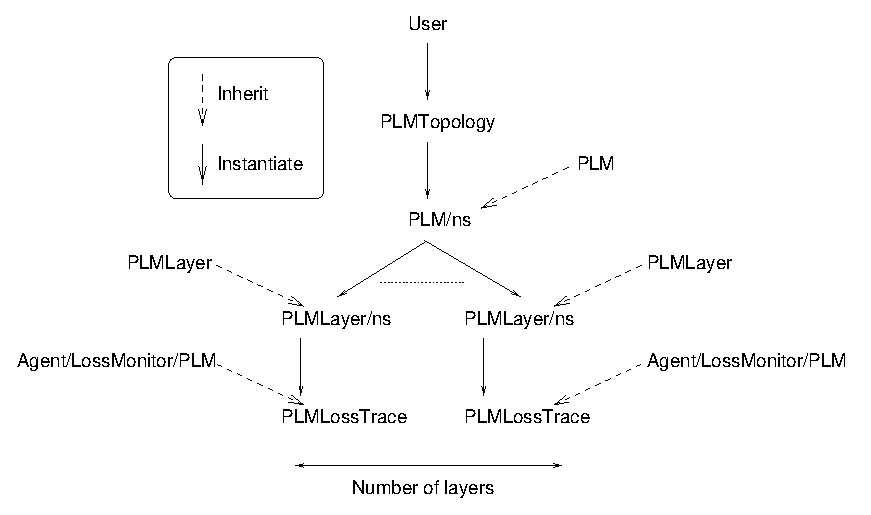
\includegraphics{instanPLMrecv.eps}}
  \caption{Inheritance and instantiation when we create a receiver.}
  \label{fig:instanPLMrecv}
\end{figure}

All the PLM machinery is implemented at the receiver. In this section we decribe
the instantiation process of a receiver. To create, place at node
{\tt n},  attach to source {\tt S}, and start at {\tt t$_1$} a PLM receiver we
call the PLMTopology instproc {\tt 
  build\_receiver n addr t$_1$ C} where {\tt addr} is the address returned
by {\tt place\_source} when {\tt S} was created, and {\tt C} is the check value. The
receiver created by {\tt build\_receiver} is an instance of the class PLM/ns,
the ns interface to the PLM 
machinery. At the initialisation of the receiver, the PLM instproc {\tt init} is
called due to inheritance. {\tt init} calls the PLM/ns instproc
{\tt create-layer} and, by this way,  creates as many instances of the class 
PLMLayer/ns (the ns interface to the PLMLayer class) as there are layers. Each
instance of PLMLayer/ns creates an instance of the class PLMLossTrace which is
reponsible for 
monitoring the received and lost packets thanks to the fact that the class
PLMLossTrace inherits from the class Agent/LossMonitor/PLM. 
Fig.~\ref{fig:instanPLMrecv} schematically describes the process  of a PLM
receiver instantiation. In the following we describe the behavior of a PLM
receiver when it receives a packet and when it detects a loss.



\subsection{Reception of a Packet}
\label{sec:PLMReception-Packet}
We create a new c++ class PLMLossMonitor (\nsf{plm/loss-monitor-plm.cc}) that
inherits from LossMonitor. The OTcl class name of the c++ PLMLossMonitor class is
Agent/LossMonitor/PLM.
\begin{program}
class PLMLossMonitor : public LossMonitor {
public:
        PLMLossMonitor();
        virtual void recv(Packet* pkt, Handler*);
protected:
        // PLM only
        int flag_PP_;
        double packet_time_PP_;
        int fid_PP_;
};

static class PLMLossMonitorClass : public TclClass {
public:
        PLMLossMonitorClass() : TclClass("Agent/LossMonitor/PLM") {}
        TclObject* create(int, const char*const*) {
                return (new PLMLossMonitor());
        }
} class_loss_mon_plm;

\end{program}

We add in {\tt void PLMLossMonitor::recv(Packet* pkt, Handler*)} a Tcl call to the
  Agent/LossMonitor/PLM instproc {\tt log-PP} each time a packet is received :
\begin{program}
  void LossMonitor::recv(Packet* pkt, Handler*)
  {
    ...
    if (expected_ >= 0) {
      ...
      }
    Tcl::instance().evalf("%s log-PP", name());
    }
\end{program}

The Agent/LossMonitor/PLM instproc {\tt log-PP} is empty. In fact, we define the {\tt
  log-PP} instproc for the class PLMLossTrace. {\tt log-PP}
computes an estimate of the available bandwidth based on a single PP burst (of
length {\tt PP\_burst\_length} in packets). Once {\tt log-PP} has received the 
  {\tt PP\_burst\_length} packets of the burst, it computes the estimate and
  calls the PLM instproc {\tt make\_estimate} with the computed estimate as
  argument. 

{\tt make\_estimate} puts the estimate based on a single PP
({\tt PP\_value}) in an array of  estimate samples ({\tt PP\_estimate}). If {\tt
  PP\_value} is lower than the current subscription level (i.e.~lower than the
throughput achieved according to the current number of layers subscribed), {\tt
  make\_estimate} calls the PLM instproc {\tt stability-drop} which simply drops
layers until the current subscription level becomes lower than {\tt PP\_value}.
{\tt make\_estimate} makes an estimate {\tt PP\_estimate\_value} by taking the
minimum {\tt PP\_value} received during the last {\tt check\_estimate} period
(if there are at
least {\tt PP\_estimation\_length} single PP estimate received). Once {\tt
  make\_estimate} has a {\tt PP\_estimate\_value} it calls the PLM instproc {\tt
  choose\_layer} which joins or drops layer(s) according to the current subscription
level and to the {\tt PP\_estimate\_value}. For details about the PLM instproc
\code{make_estimate}, refer to its code in \nsf{tcl/plm/plm.tcl}.



\subsection{Detection of a Loss}
Each time a loss is detected by an instance of the class PLMLossMonitor, a call to
the Agent/LossMonitor/PLM instproc {\tt log-loss} is triggered. The
Agent/LossMonitor/PLM instproc {\tt log-loss} 
is empty. In fact, we define the {\tt log-loss} instproc for the class
PLMLossTrace. The PLMLossTrace instproc {\tt log-loss} simply
calls the PLM instproc {\tt log-loss} which contains the PLM machinery in case
of loss. In summary, {\tt log-loss} only drops a layer when the loss rate
exceeds 10\% (this test is executed by the PLM instproc {\tt
  exeed\_loss\_thresh}). After a layer drop {\tt log-loss} precludes any
other layer drop due to loss for 500ms. For details about the PLM instproc {\tt
  log-loss}, refer to its code in \nsf{tcl/plm/plm.tcl}. 

\subsection{Joining or Leaving a Layer}
To join a layer the PLM instproc {\tt add-layer} is called. This instproc
calls the PLMLayer instproc {\tt join-group} which calls the PLMLayer/ns instproc {\tt
  join-group}.
To leave a layer the PLM instproc {\tt drop-layer} is called. This instproc
calls the PLMLayer instproc {\tt leave-group} which calls the PLMLayer/ns instproc {\tt
  leave-group}.

\section{Commands at a Glance}
Note: This section is a copy paste of the end of
section~\ref{sec:Configuration}. We add this section to preserve homogeneity with
the ns manual.

All the simulations for PLM should be set using the PLMTopology environment (as
in the example script where we define a PLMTopology superclass called Scenario0). The
user interface is (all the instproc can be found in \nsf{tcl/plm/plm-topo.tcl}):
\begin{description}
\item[\tt build\_link a b d bw] creates a duplex link between node
  \code{a} and \code{b} with a delay \code{d} and a bandwidth \code{bw}. If
  either node does not exist, \code{build_link} creates it.
\item[\tt place\_source n t] creates and places a PLM source at node \code{n} and
  starts it at time \code{t}. \code{place_source} returns \code{addr} which
  allows to attach receivers to this source.
\item[\tt place\_receiver n addr C nb] creates and places a PLM receiver at node
  \code{n} and attached it to the source which return the address \code{addr}. The
  check value for this PLM receiver is \code{C}. An optional parameter \code{nb}
  allows to get an instance of the PLM receiver called \code{PLMrcvr($nb)}. This
  instance is only useful to get some specific statistics about this receiver
  (mainly the number of packets received or lost). %$
\end{description}
}


